\documentclass[manuscript]{copernicus}
\graphicspath{{pictures/}}          % graphics
\begin{document}
\clearpage
\setcounter{page}{1}

\section*{Supplement}
\subsection*{S.1 Dynamic viscosity of air and quasi-laminar resistance}
\subsubsection*{S.1.1 Sutherland's law and linear fits}
\appendixfigures
\begin{center}
  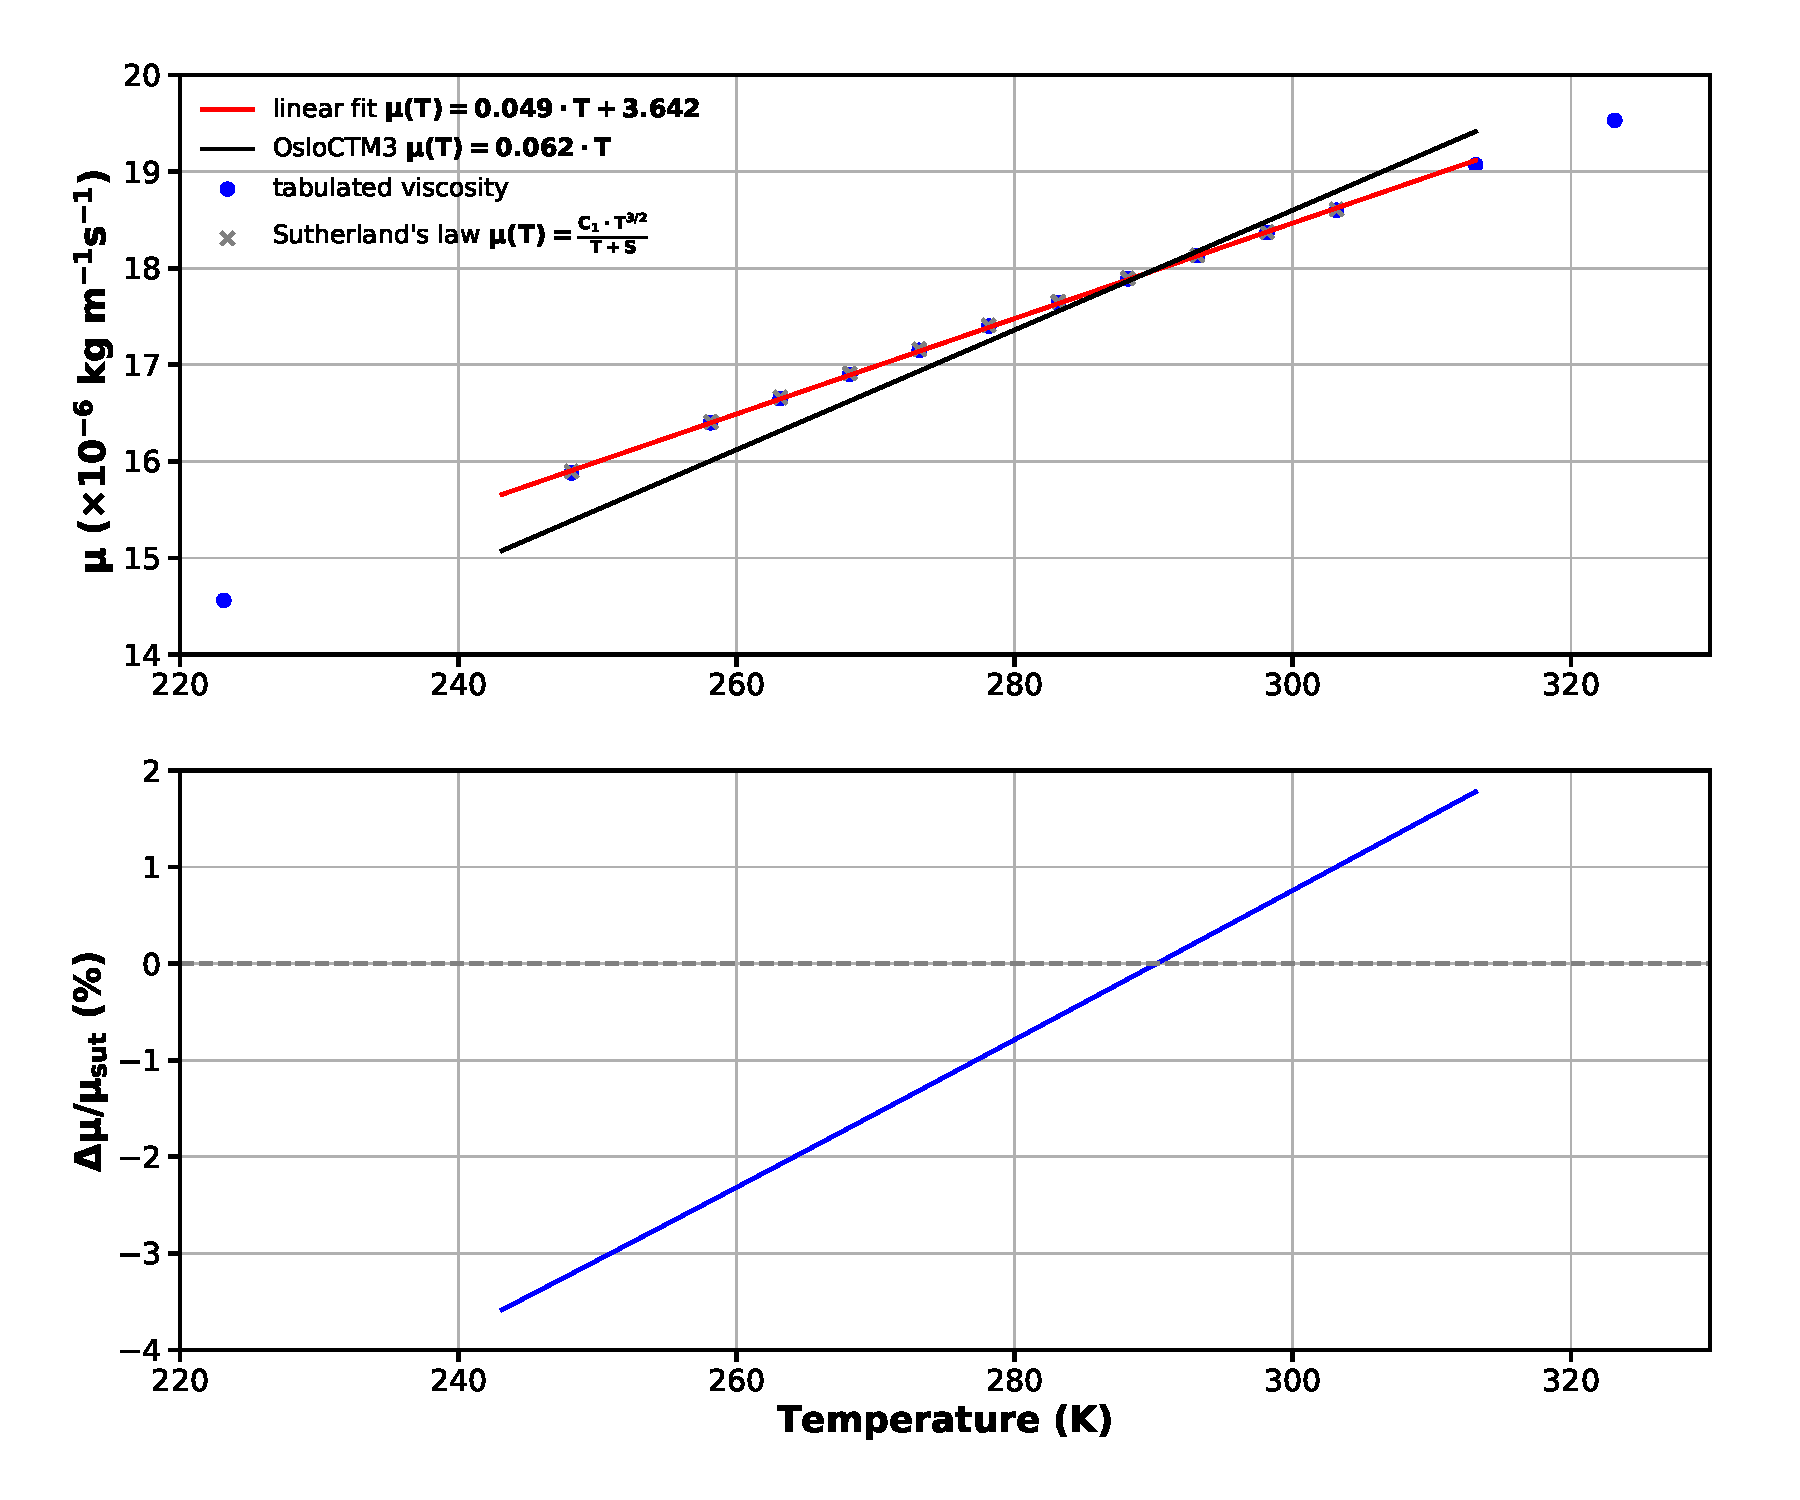
\includegraphics[height=0.4\textheight]{pictures/dynamic_viscosity.pdf}
\end{center}
\subsubsection*{S.1.2 Comparison of $z_o$ and $R_b$ for $\mu(T) = m\cdot T$ and Sutherland's law: \chem{H_2O}}
\appendixfigures
\begin{center}
  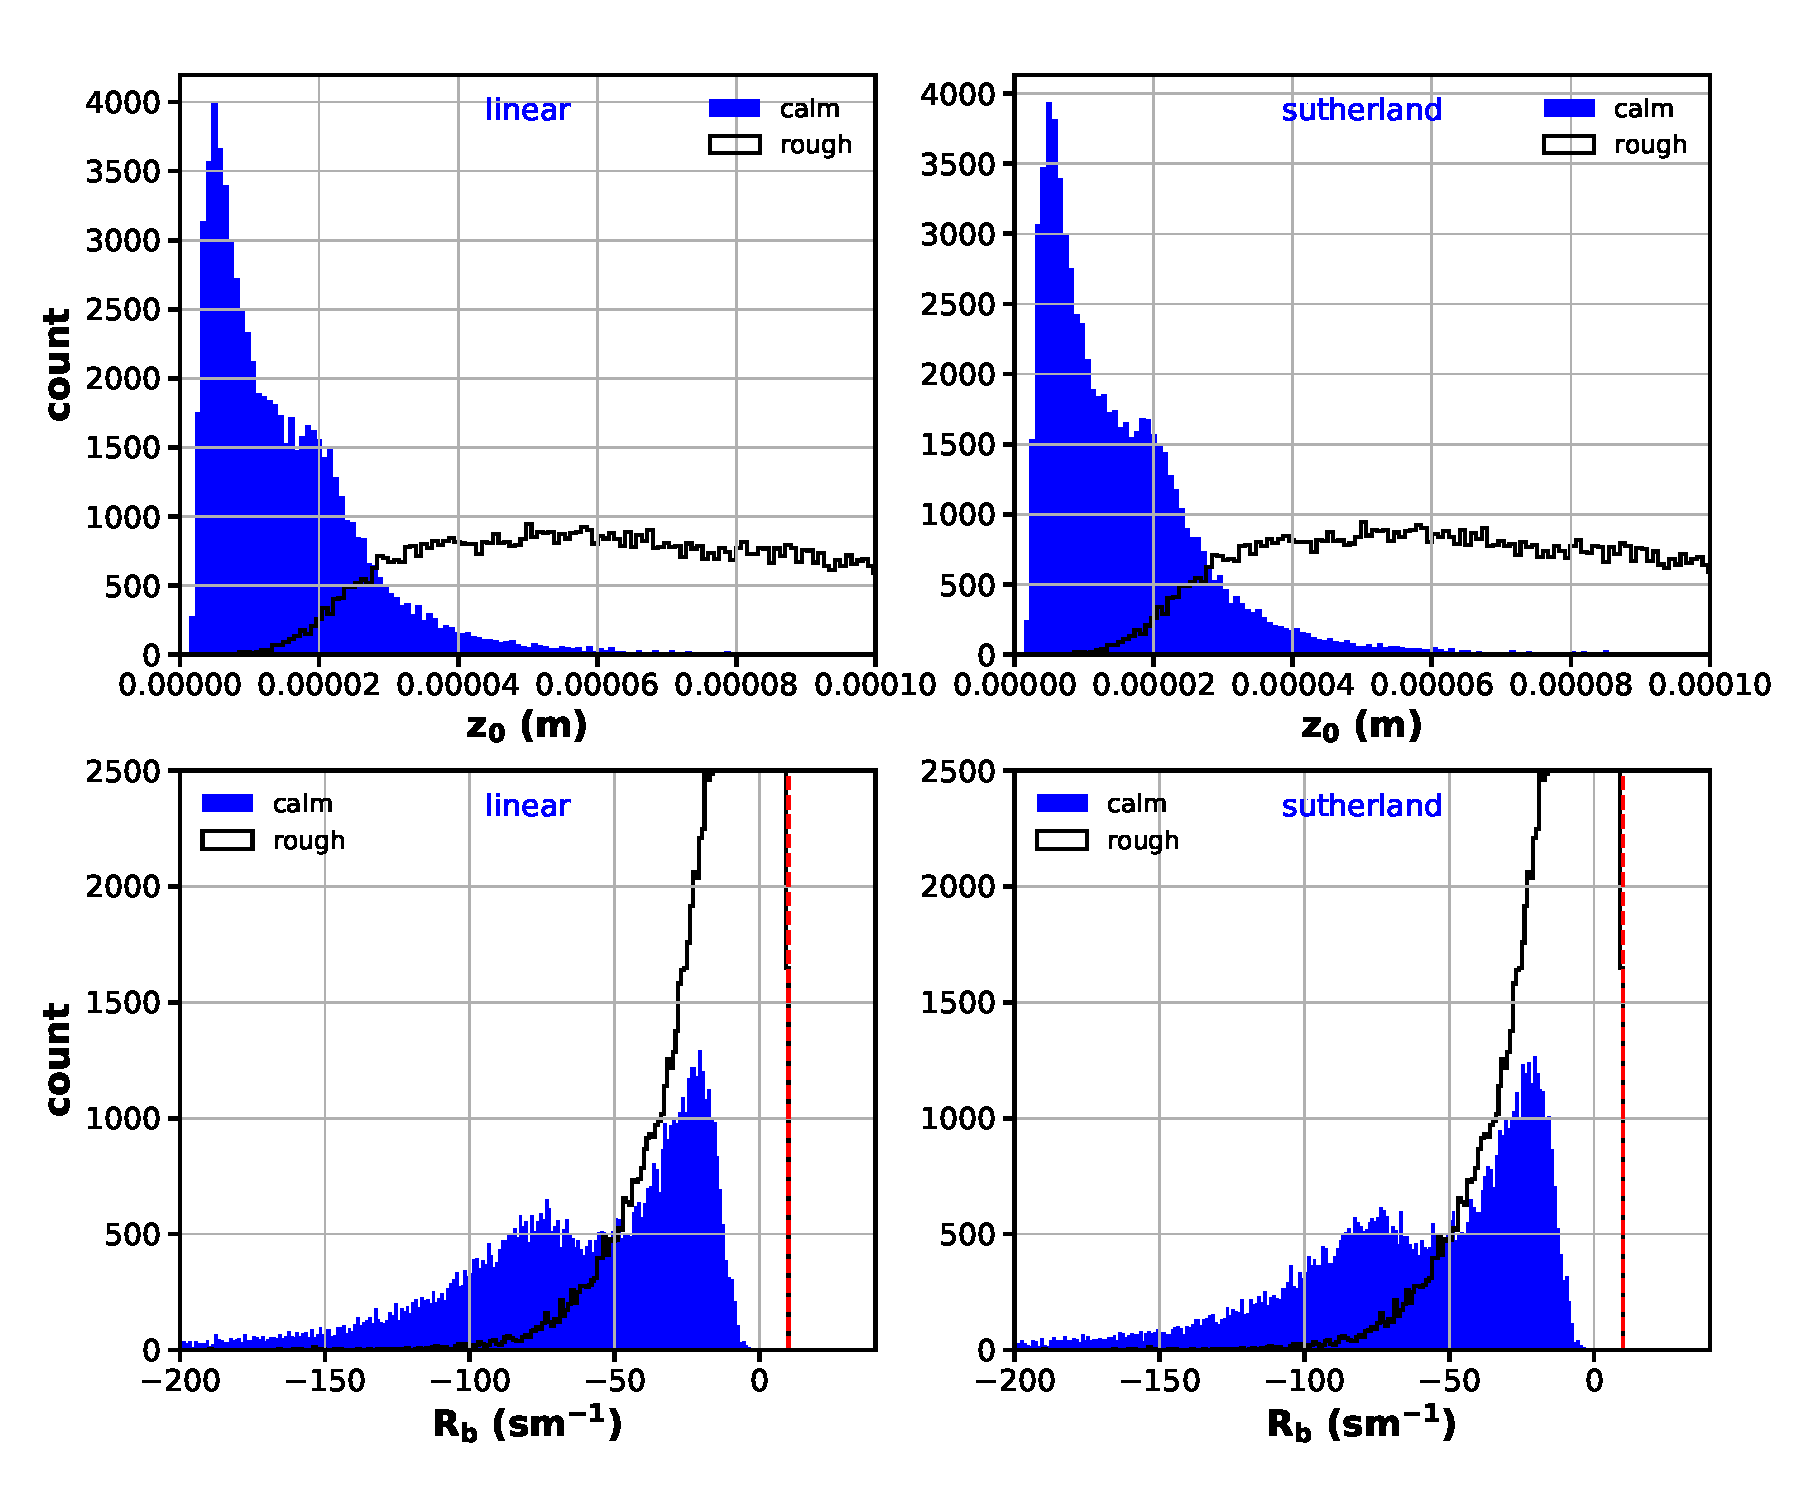
\includegraphics[height=0.4\textheight]{pictures/dynamic_viscosity_zo_Rb.pdf}
\end{center}
\subsubsection*{S.1.3 $R_b$ for different species}
\appendixfigures
\begin{center}
  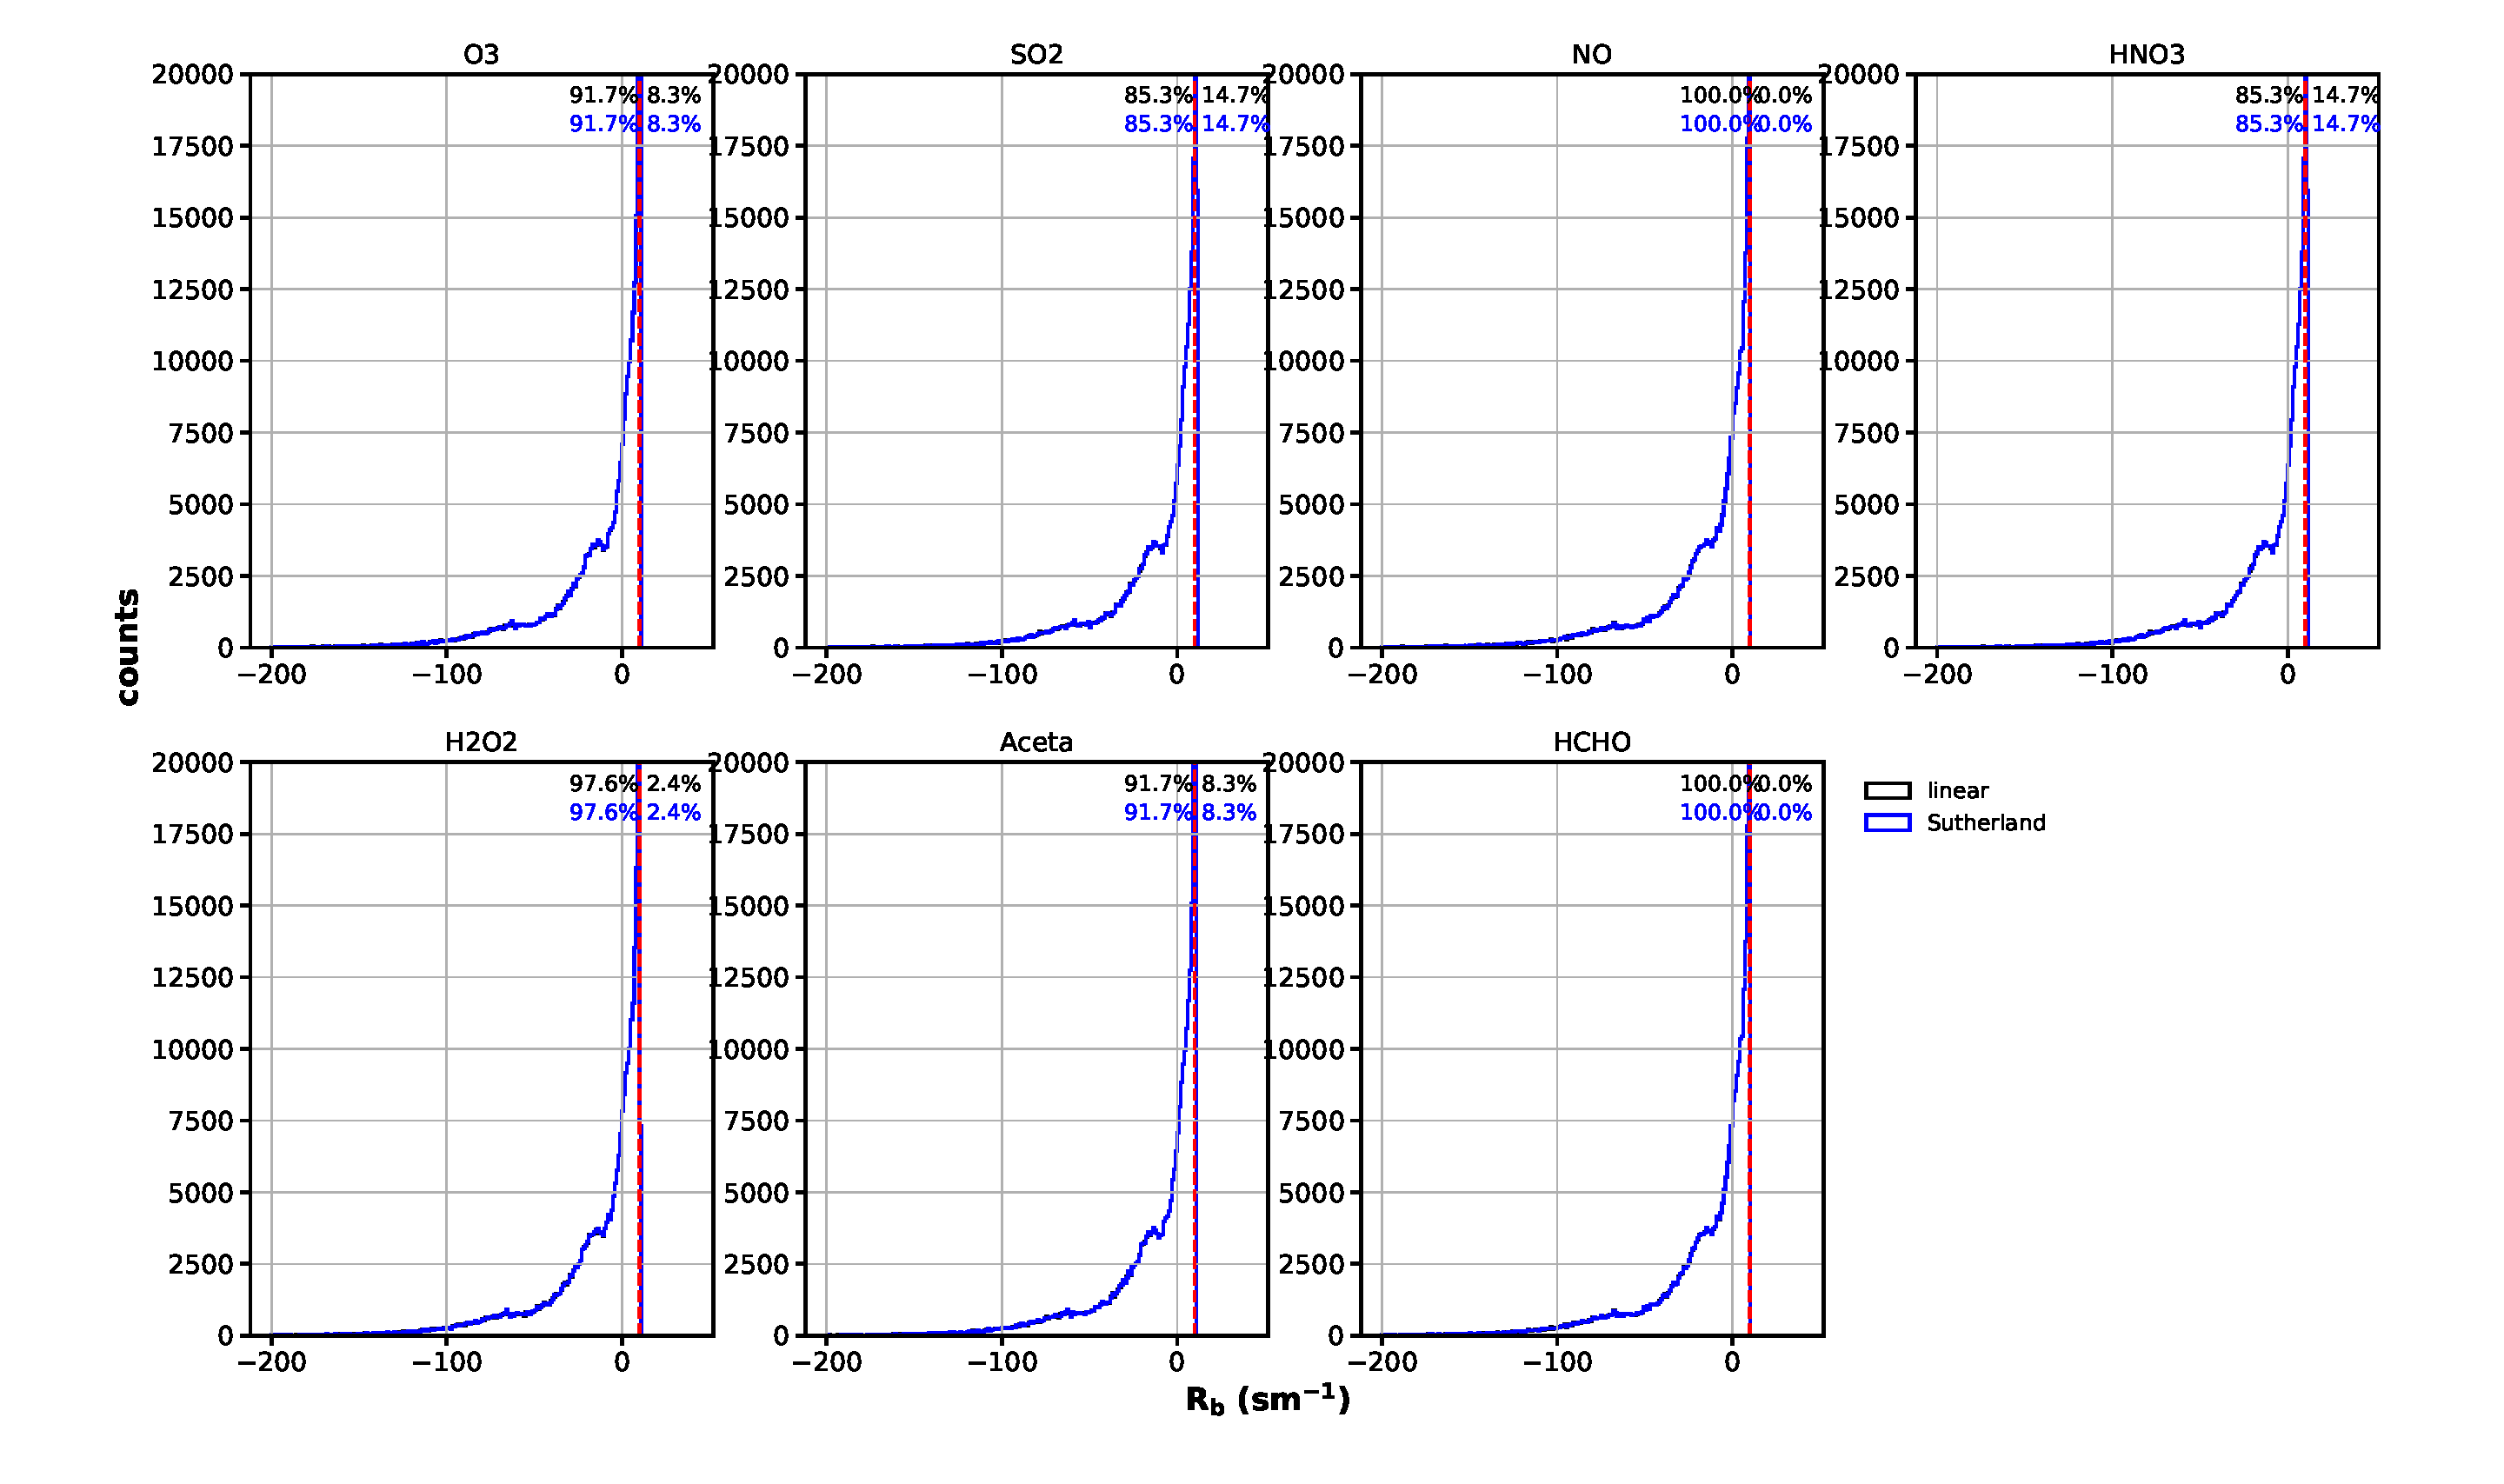
\includegraphics[height=0.45\textheight]{pictures/dynamic_viscosity_Rbi_1.pdf}
  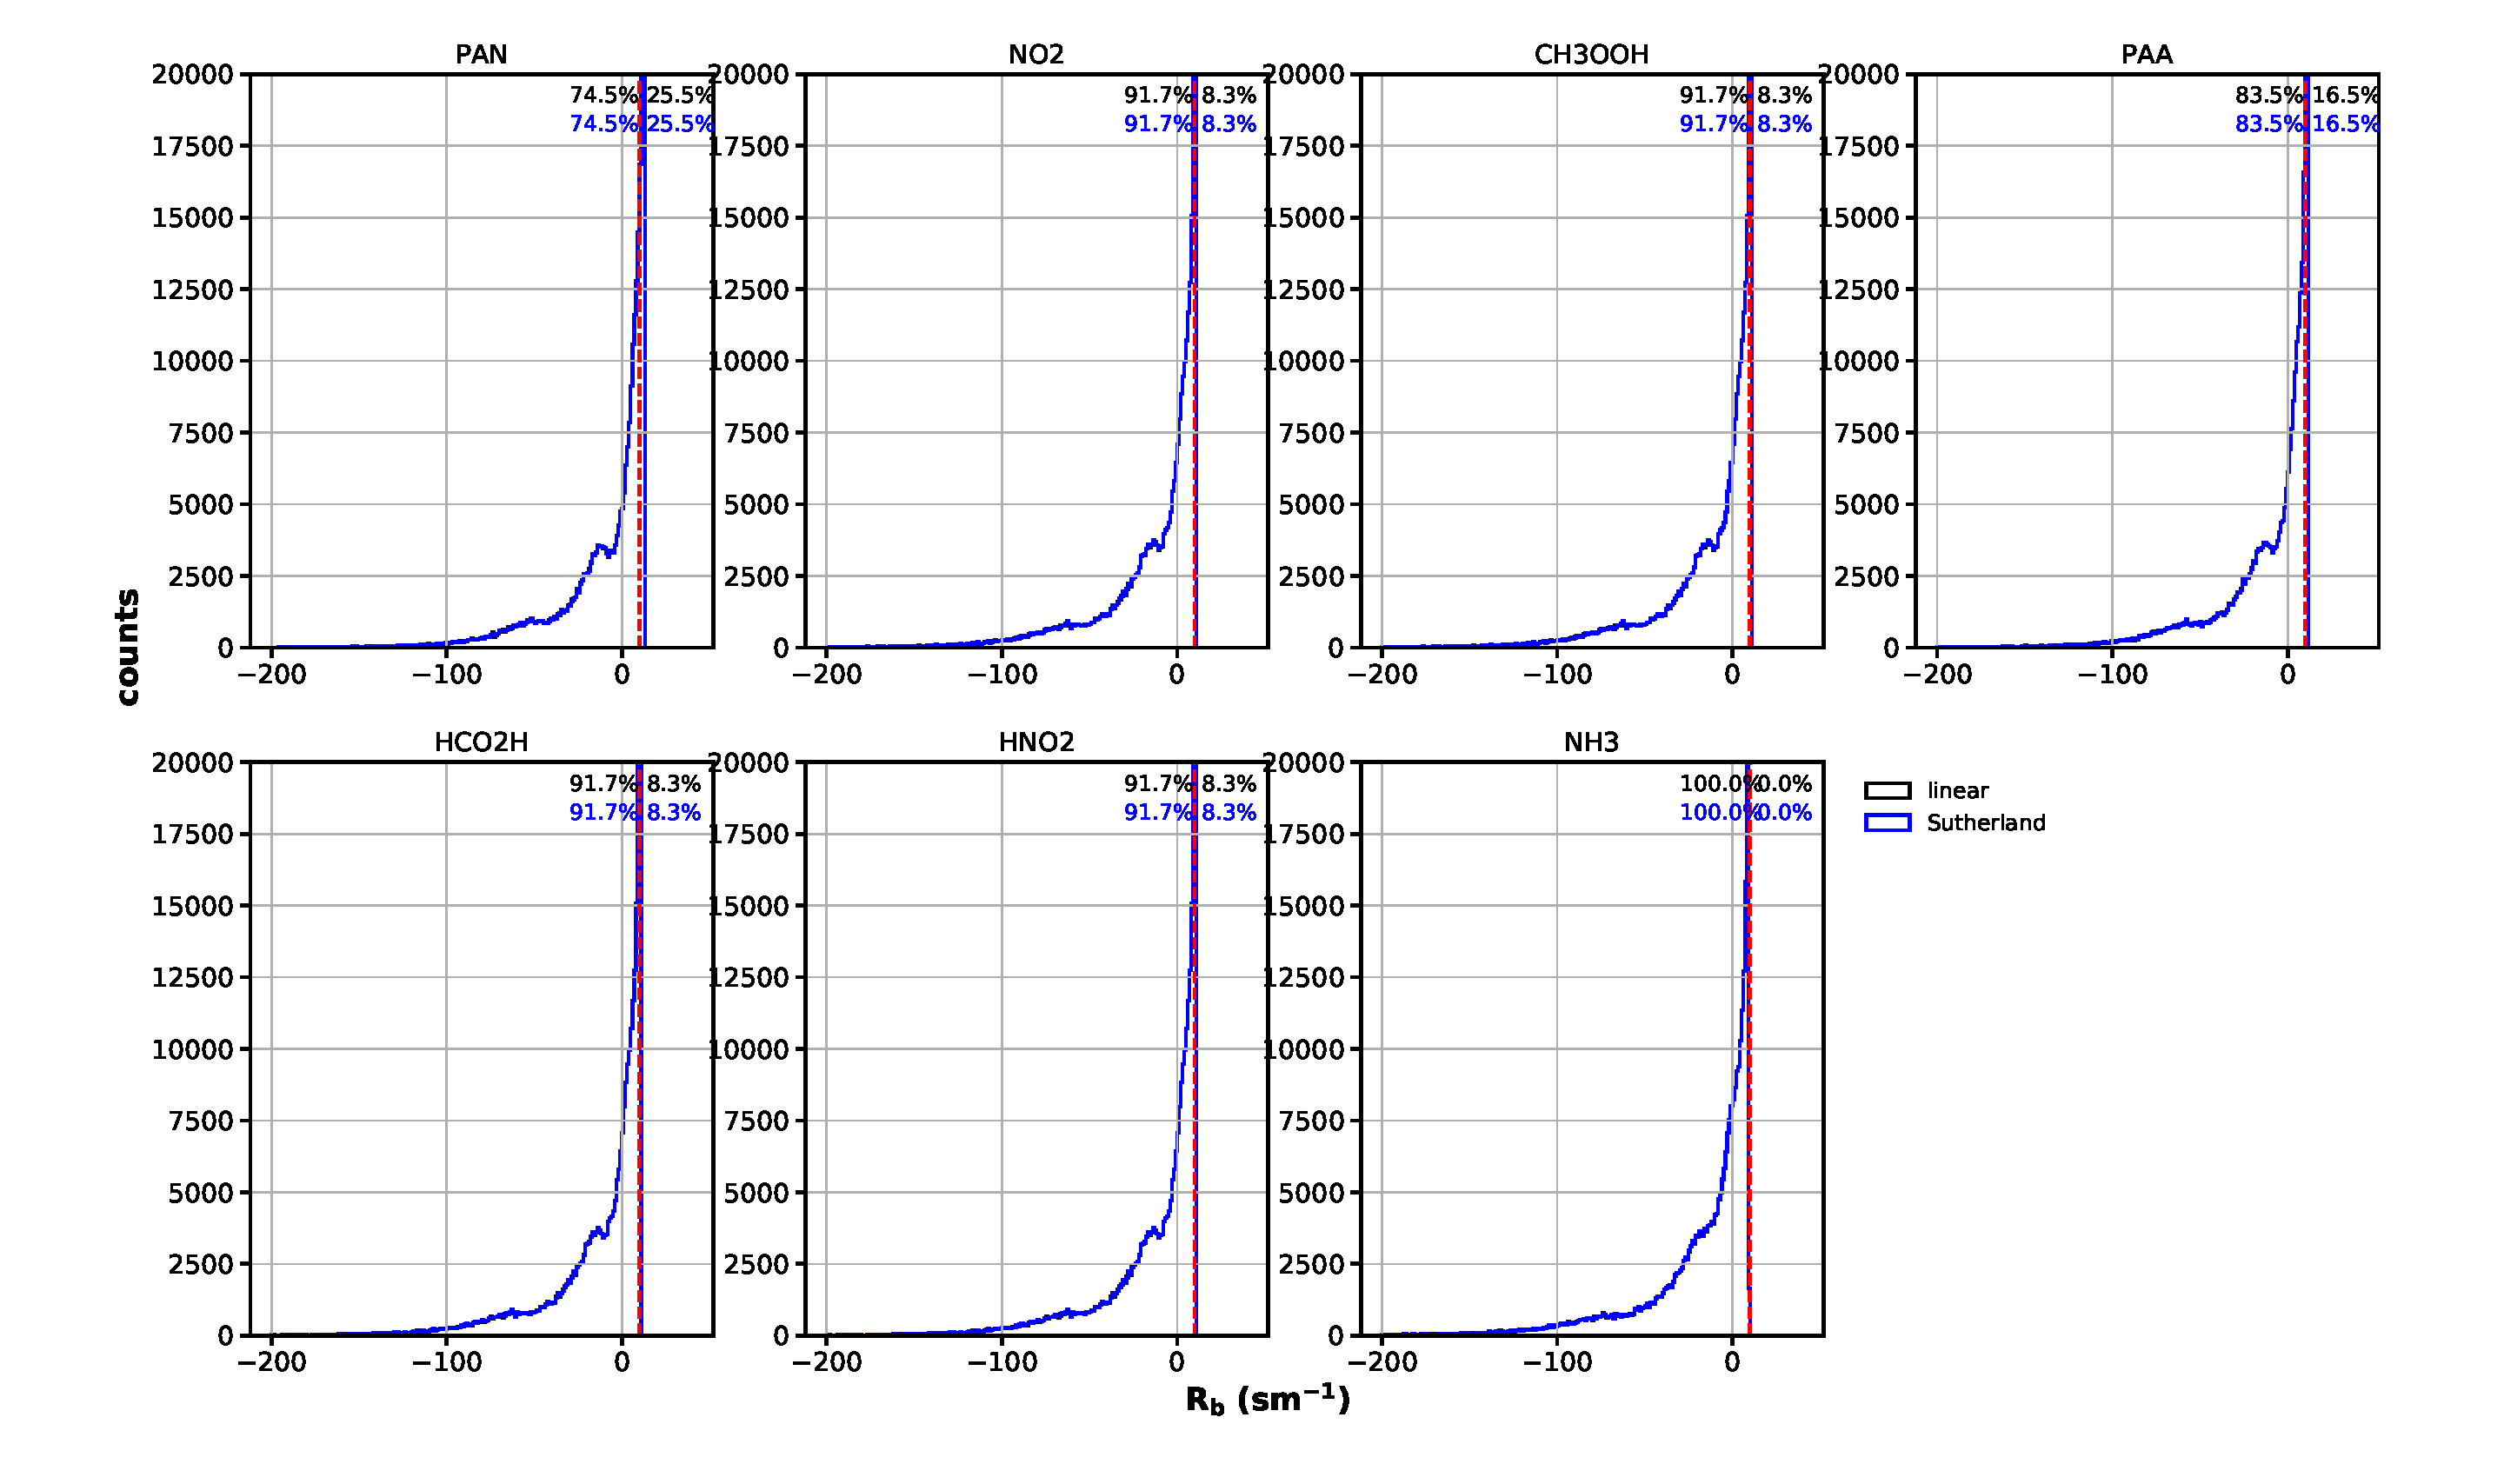
\includegraphics[height=0.45\textheight]{pictures/dynamic_viscosity_Rbi_2.pdf}
\end{center}

%\begin{minipage}[t]{1.\textwidth}
\subsection*{S.2 Tabulated parameters for stomatal conductance}
\appendixtables
\begin{sidewaystable}[!htbp]
  %\caption{S.2 Tabulated parameters for stomatal conductance}
  \begin{tabular}{lcccccccccccccc}
    \tophline
    Code & $g_\text{max}$ & $f_\text{min}$ & $\phi_a$ & $\phi_b$ & $\phi_c$ & $\phi_d$ & $\phi_e$ & $\phi_f$ & $\phi_\text{AS}$ & $\phi_\text{AE}$ & $f_\text{light}$ & $T_\text{min}$ & $T_\text{opt}$ & $T_\text{max}$ \\
    &&&&&&&&&&&&&&\\
    \middlehline
    CF & 140 & 0.1 & 0.8 & 0.8 & 0.8 & 0.8 & 1 & 1 & 0 & 0 & 0.006 & 0 & 18 & 36  \\
    DF & 150 & 0.1 & 0 & 0 & 1 & 0 & 20 & 30 & 0 & 0 & 0.006 & 0 & 20 & 35  \\
    NF & 200 & 0.1 & 1 & 1 & 0.2 & 1 & 130 & 60 & 80 & 35 & 0.013 & 8 & 25 & 38 \\
    BF & 200 & 0.02 & 1 & 1 & 0.3 & 1 & 130 & 60 & 80 & 35 & 0.009 & 1 & 23 & 39 \\
    TC & 300 & 0.1 & 0.1 & 1 & 0.1 & 0 & 45 & 0 & 0 & 0.0105 & 0.01 & 12 & 26 & 40 \\
    MC & 300 & 0.019 & 0.1 & 0.1 & 1 & 0.1 & 0 & 45 & 0 & 0 & 0.0048 & 0 & 25 & 51  \\
    RC & 360 & 0.02 & 0.2 & 0.2 & 1 & 0.2 & 20 & 45 & 0 & 0 & 0.0023 & 8 & 24 & 50  \\
    SNL & 60 & 0.01 & 1 & 1 & 1 & 1 & 1 & 1 & 0 & 0 & 0.009 & 1 & 18 & 36 \\
    GR & 270 & 0.01 & 1 & 1 & 1 & 1 & 0 & 0 & 0 & 0 & 0.009 & 12 & 26 & 40 \\
    MS & 200 & 0.01 & 1 & 1 & 0.2 & 1 & 130 & 60 & 80 & 35 & 0.012 & 4 & 20 & 37 \\
    WE & 0 & 1 & 1 & 1 & 1 & 1 & 1 & 1 & 1 & 1 & 1 & 0 & 1 & 0 \\
    TU & 0 & 1 & 1 & 1 & 1 & 1 & 1 & 1 & 1 & 1 & 1 & 0 & 1 & 0  \\
    DE & 0 & 1 & 1 & 1 & 1 & 1 & 1 & 1 & 1 & 1 & 1 & 0 & 1 & 0  \\
    W & 0 & 1 & 1 & 1 & 1 & 1 & 1 & 1 & 1 & 1 & 1 & 0 & 1 & 0 \\
    ICE & 0 & 1 & 1 & 1 & 1 & 1 & 1 & 1 & 1 & 1 & 1 & 0 & 1 & 0 \\
    U & 0 & 1 & 1 & 1 & 1 & 1 & 1 & 1 & 1 & 1 & 1 & 0 & 1 & 0 \\
    \bottomhline
  \end{tabular}
  \\
  \vspace{2\baselineskip}
  \begin{tabular}{lcccccccccccccc}
    \tophline
    Code & $D_\text{max}$ & $D_\text{min}$ & $D_\text{crit}$ & $R_\chem{SO}$ & $R_\chem{O_3}$ & height & $d_\text{SGS}$ & $d_\text{EGS}$ & $\nabla d_\text{SGS}$ & $\nabla d_\text{EGS}$ & $\text{LAI}_\text{min}$ & $\text{LAI}_\text{max}$ & LS & LE \\
    &&&&&&&&&&&&&& \\
    \middlehline
    CF & 0.5 & 3 & 1000 & 0 & 200 & 20 & 0 & 366 & 0 & 0 & 5 & 5 & 1 & 1\\
    DF & 1 & 3.25 & 1000 & 0 & 200 & 20 & 100 & 307 & 1.5 & -2.0 & 0 & 4 & 20 & 30\\
    NF & 1 & 3.2 & 1000 & 0 & 200 & 8 & 0 & 366 & 0 & 0 & 4 & 4 & 1 & 1\\
    BF & 2.2 & 4 & 1000 & 0 & 200 & 15 & 0 & 366 & 0 & 0 & 4 & 4 & 1 & 1\\
    TC & 1.2 & 3.2 & 8 & 0 & 200 & 1 & 123 & 213 & 2.57 & 2.57 & 0 & 3.5 & 70 & 20\\
    MC & 1 & 2.5 & 1000 & 0 & 200 & 2 & 123 & 237 & 2.57 & 2.57 & 0 & 3 & 70 & 44\\
    RC & 0.31 & 2.7 & 10 & 0 & 200 & 1 & 130 & 250 & 0 & 0 & 0 & 4.2 & 35 & 65\\
    SNL & 1.3 & 3 & 1000 & 0 & 400 & 0.5 & 0 & 366 & 0 & 0 & 2 & 3 & 192 & 96\\
    GR & 1.3 & 3 & 1000 & 0 & 1000 & 0.3 & 0 & 366 & 0 & 0 & 2 & 3.5 & 140 & 135\\
    MS & 1.3 & 3.2 & 1000 & 0 & 200 & 2 & 0 & 366 & 0 & 0 & 2.5 & 2.5 & 1 & 1\\
    WE  & 1 & 0 & 1000 & 50 & 400 & 0.5 & 0 & 366 & 0 & 0 & 0 & 0 & 0 & 0\\
    TU & 1 & 0 & 1000 & 500 & 400 & 0.5 & 0 & 366 & 0 & 0 & 0 & 0 & 0 & 0\\
    DE & 1 & 0 & 1000 & 1000 & 2000 & 0 & 0 & 366 & 0 & 0 & 0 & 0 & 0 & 0\\
    W  & 1 & 0 & 1000 & 1 & 2000 & 0 & 0 & 366 & 0 & 0 & 0 & 0 & 0 & 0\\
    ICE & 1 & 0 & 1000 & 1000 & 2000 & 0 & 0 & 366 & 0 & 0 & 0 & 0 & 0 & 0\\
    U & 1 & 0 & 1000 & 400 & 400 & 10 & 0 & 366 & 0 & 0 & 0 & 0 & 0 & 0\\
    \bottomhline
  \end{tabular}
\end{sidewaystable}
%\end{minipage}

\subsection*{S.3 Latitude dependent vegetation height}
\appendixfigures
\begin{center}
  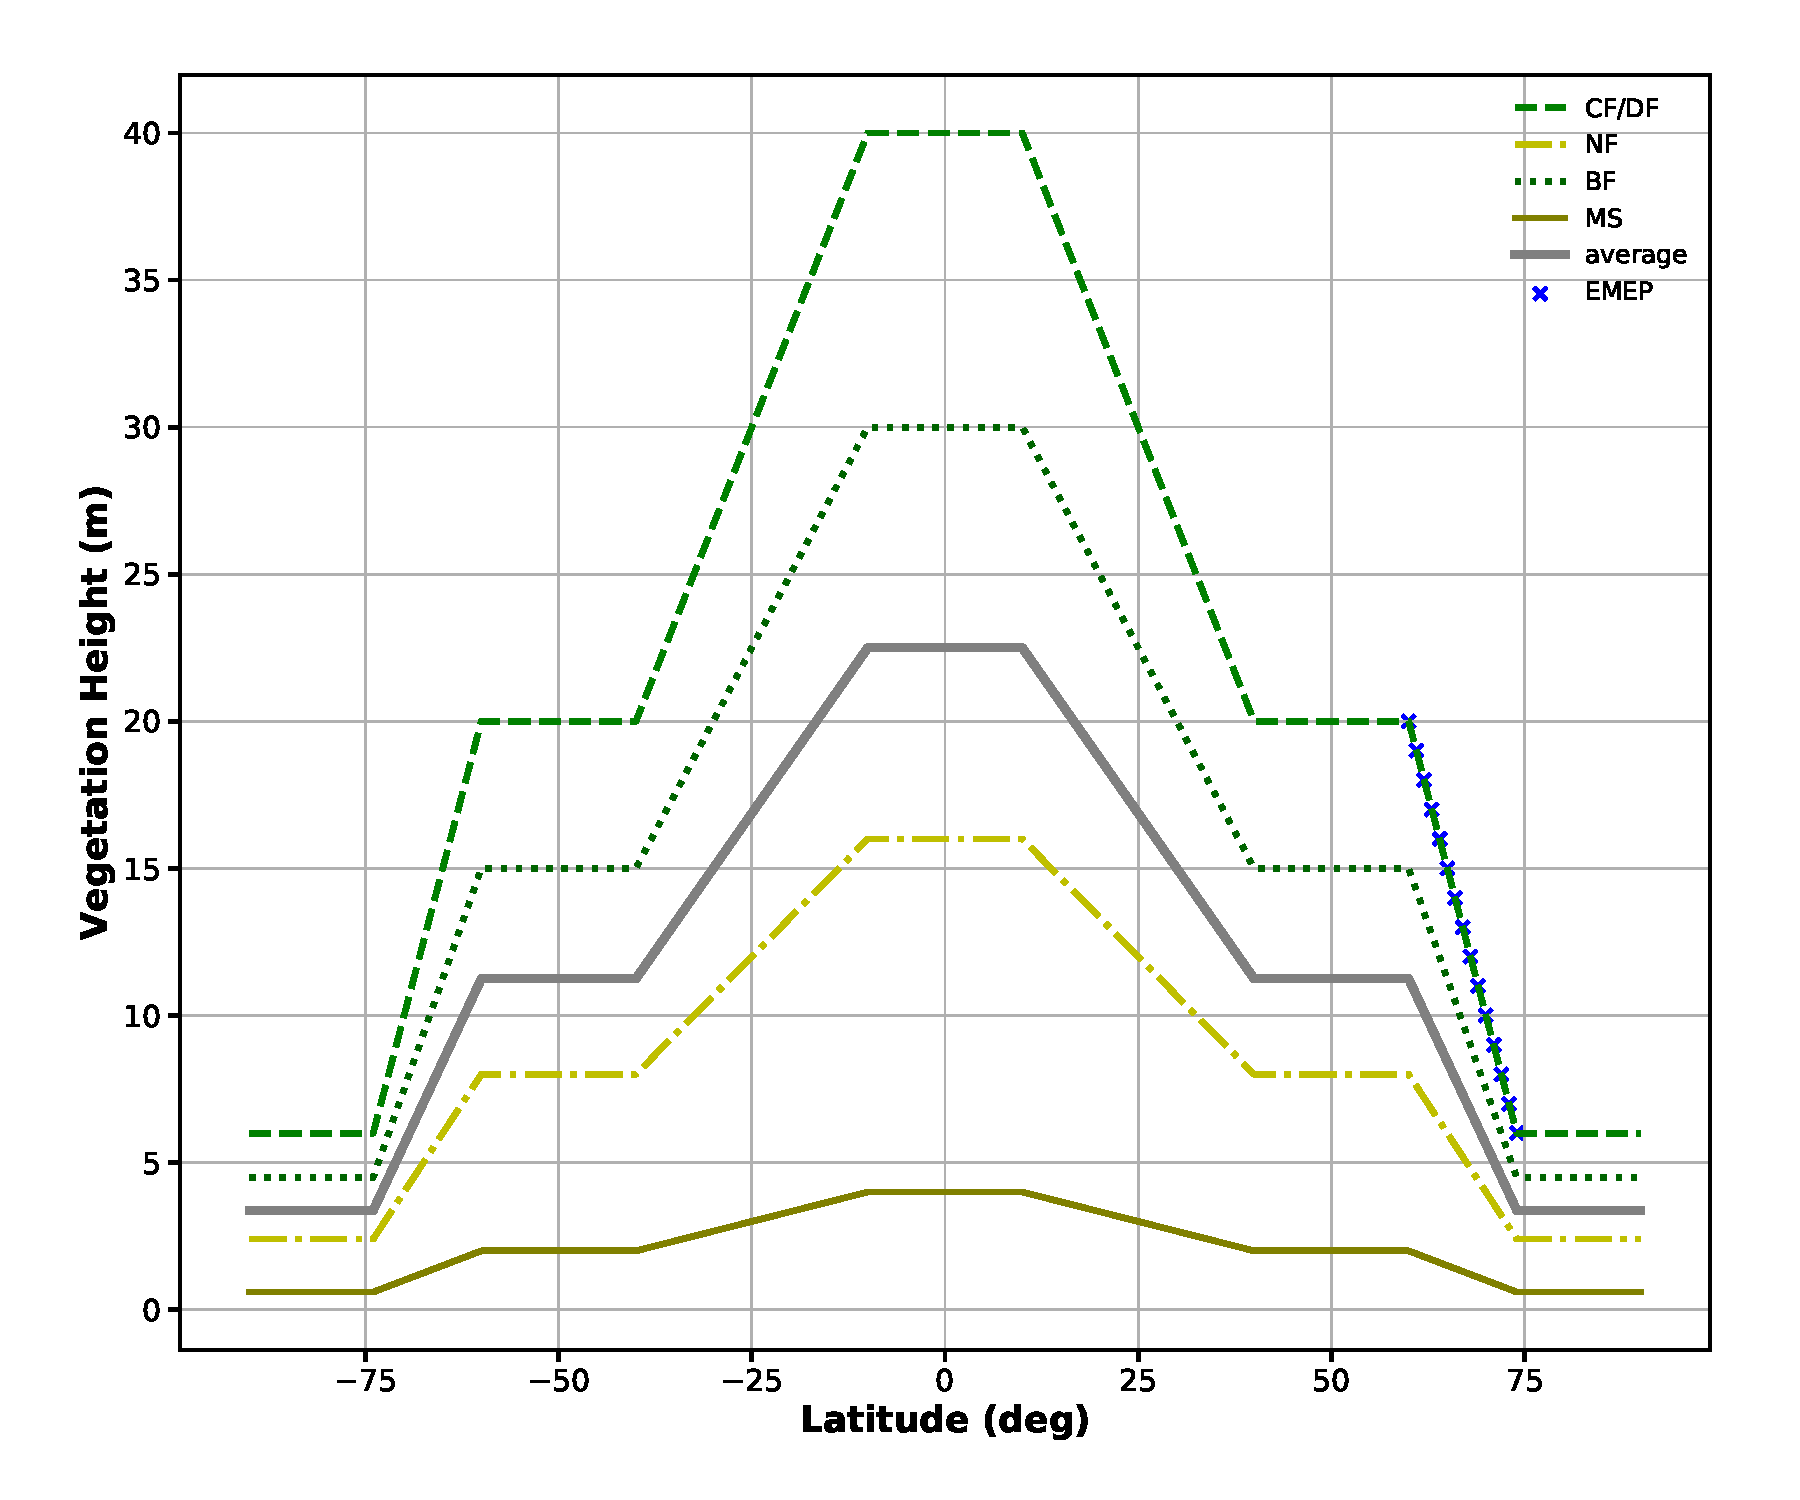
\includegraphics[height=0.4\textheight]{pictures/tree_height.pdf}
\end{center}

\subsection*{S.4 De-accumulation of photoactive radiation (PAR) from OpenIFS: January 1st 2005}
\subsubsection*{S.4.1 Output from OpenIFS: Accumulated PAR}
\appendixfigures
\begin{center}
  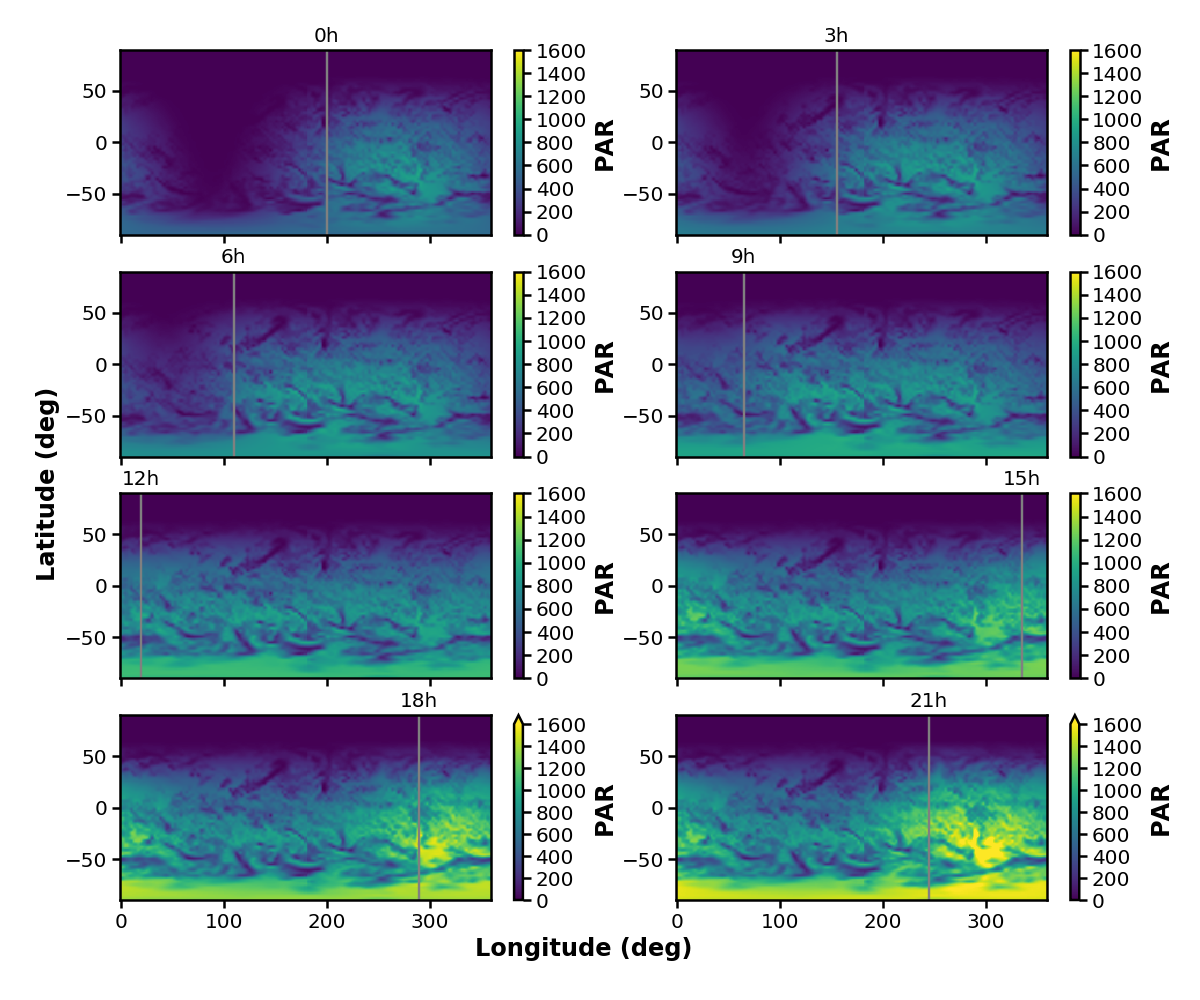
\includegraphics[height=0.4\textheight]{pictures/PAR_as_is.png}
\end{center}
\subsubsection*{S.4.2 Partly de-accumulated}
\appendixfigures
\begin{center}
  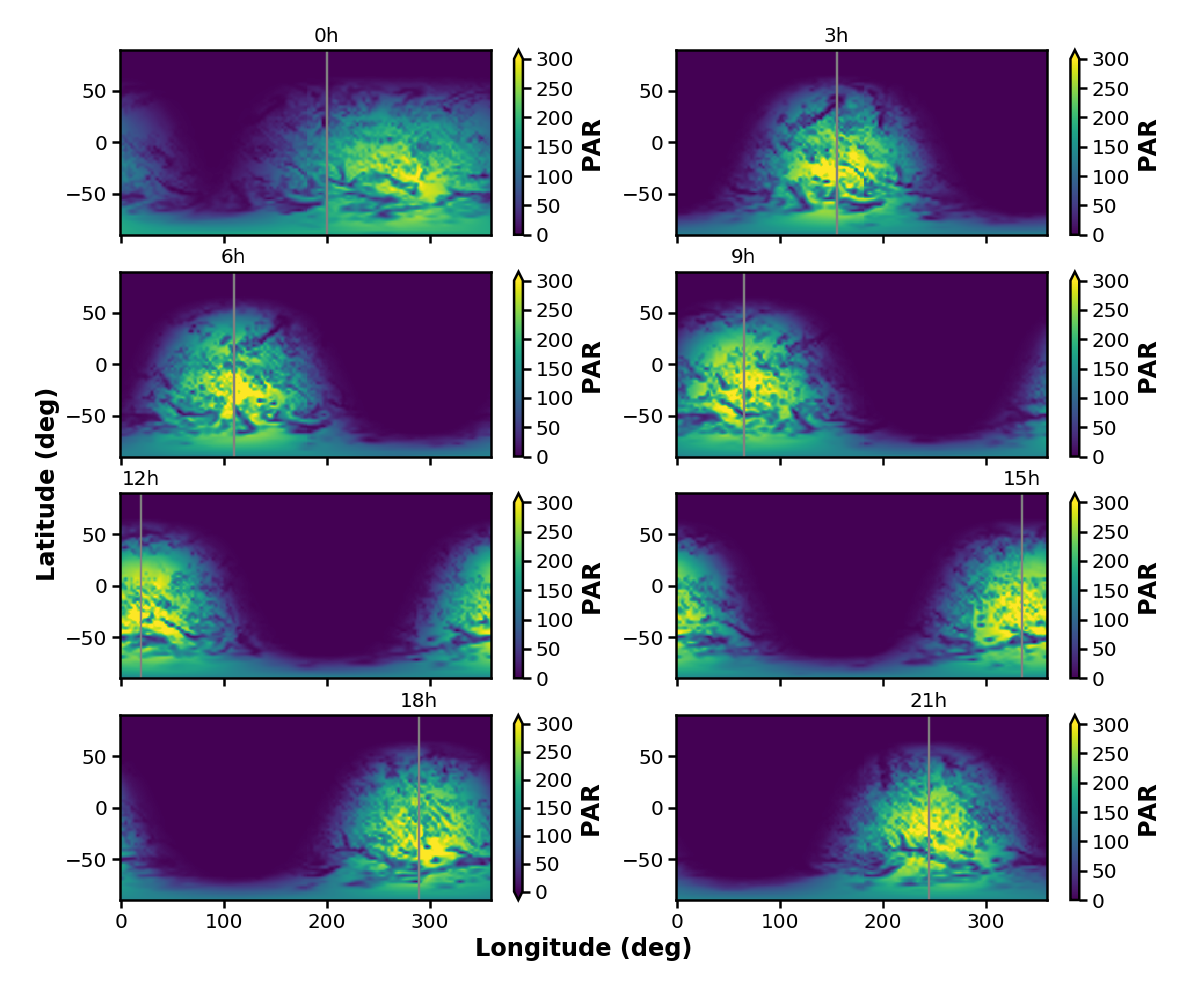
\includegraphics[height=0.4\textheight]{pictures/PAR_partly_deaccumulated.png}
\end{center}
\subsubsection*{S.4.3 De-accumulation of hour 00}
\appendixfigures
\begin{center}
  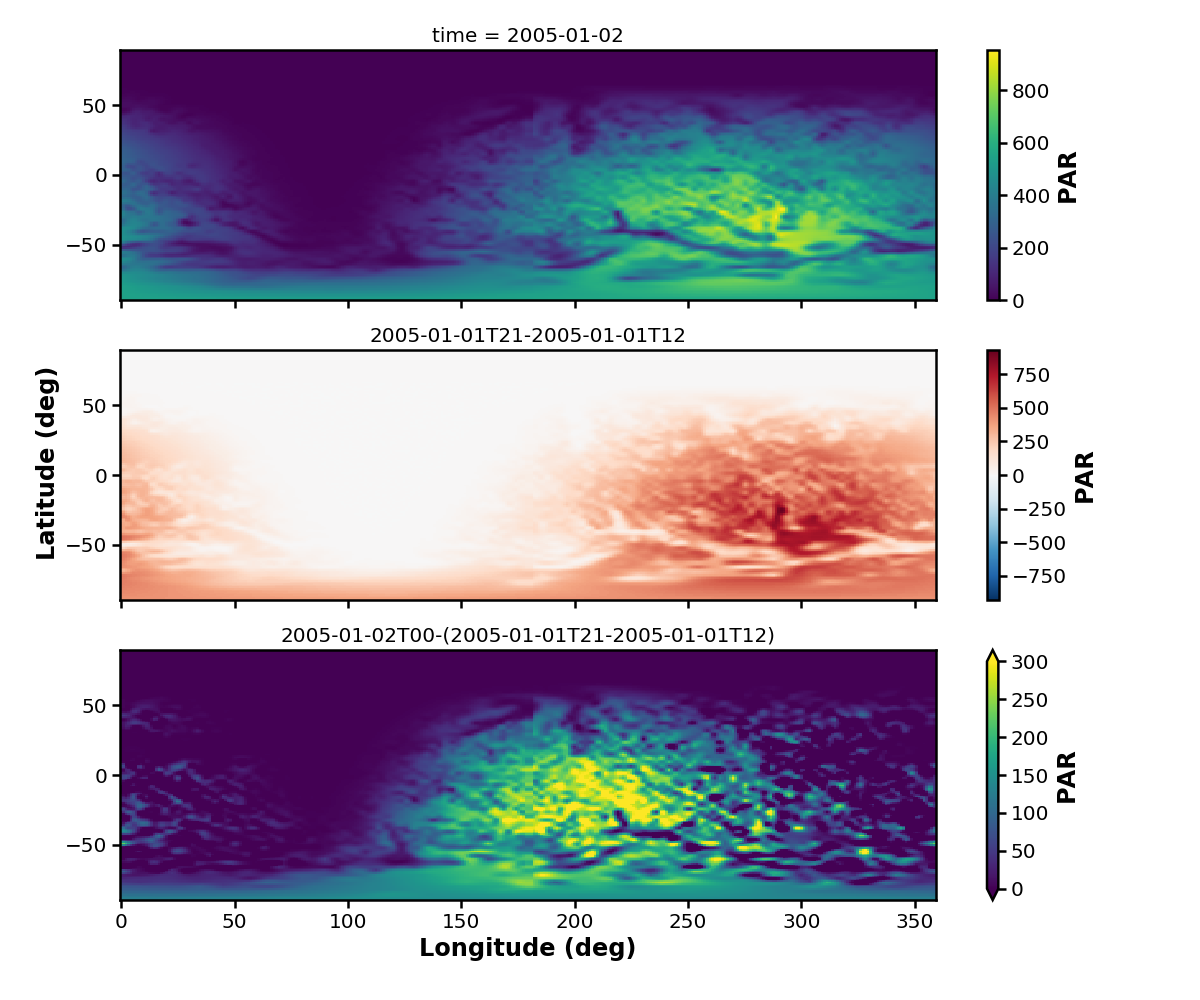
\includegraphics[height=0.4\textheight]{pictures/PAR_deaccumulating_00h.png}
\end{center}

\end{document}
